\documentclass[a4paper,10pt]{beamer}


\usepackage[utf8]{inputenc}
\usepackage{polski}
\usepackage[OT4,T1]{fontenc}
\usepackage{amsmath}
\usepackage{amsthm}
\usepackage{graphicx}
\usepackage{dsfont}
\usepackage{amssymb}
\usepackage{enumerate}
\usepackage{tikz}

\usetheme{Warsaw}
\usecolortheme{beaver}

\newtheorem{defi}{Definicja}[subsection]
\newtheorem{uw}{Uwaga}[subsection]
\newtheorem{cel}{Cel}[subsection]
\newtheorem{tw}{Twierdzenie}[subsection]
\newtheorem{lem}{Lemat}[subsection]
\newtheorem{przyk}{Przykład}[subsection]
\newtheorem{alg}{Algorytm}[subsection]

\date{14 stycznia 2016}
\title{Mobilny ankieter}
\author[A. Bohonos, D. Demski, A. Mieldzioc]{Andrzej Bohonos, Dominik Demski, Adam Mieldzioc}
\DeclareUnicodeCharacter{00A0}{ }
\begin{document}
	
	\begin{frame}
		\titlepage
	\end{frame}
	\begin{frame}{Agenda}
		\tableofcontents
	\end{frame}
	
	\section{Założenia projektu}
	\begin{frame}{Założenia projektu}
		
		\begin{itemize}
			\item tworzenie, wypełnianie i podstawowa analiza statystyczna ankiet
			\item dostępne są następujące typy pytań: pytanie jednokrotnego wyboru, wielokrotnego wyboru, wybór z listy, skala, w formie tabelki, otwarte
			\item Ankieta może być rozumiana w tradycyjny sposób jako zbiór pytań zadawanych osobom ankietowanym, ale także jako formularz do zbierania danych na przykład podczas pracy w terenie. 
			\item W skład systemu wchodzą: aplikacja mobilna na platformę Android, aplikacja desktopowa stworzona w języku Java
		\end{itemize}
	\end{frame}
	\begin{frame}{Dla kogo jest Mobilny ankieter?}
		
		\begin{itemize}
			\item dla studentów zbierających dane do prac dyplomowych 
			\item dla pracowników naukowych
			\item  dla jednostek naukowych
			\item organizacji pozarządowych
			\item  urzędów (np. do spisu ludności)
			\item dla firm, które do funkcjonowania na rynku potrzebują danych na określony temat
		\end{itemize}
		System jest przygotowany do użytkowania go zarówno przez jednego użytkownika, jak i grupę użytkowników.
	\end{frame}
	
	
	\begin{frame}{Przykładowe zastosowania systemu}
		Przykładowe zastosowania systemu:
		\begin{itemize}
			\item przeprowadzanie anonimowych ankiet (np. wśród przechodniów),
			\item przeprowadzanie spisów ludności,
			\item przeprowadzania głosowań,
			\item kontrola intalacji technicznej w zakładach przemysłowych.
		\end{itemize}
	\end{frame}
	
	\section{Zakres wstępny i co zostało osiągnięte}
	
	
	\begin{frame}{Aplikacja desktopowa}
		
		\begin{enumerate}
			\item do zrobienia – przegląd wymagań przyjętych do realizacji i zaimplementowanych w semestrze zimowym, różnice z semestrem letnim
		\end{enumerate}
	\end{frame}
	
	\begin{frame}{Aplikacja mobilna}
		\begin{enumerate}
			\item	stworzenie szablonu ankiet z różnymi typami pytań 
			\item	wypełnianie ankiety (zapisanie wyników w urządzeniu)
			\item	możliwość korzystania z tego samego szablonu ankiety na różnych urządzeniach (wczytywanie i generowanie plików .json)
			\item	sprawdzanie poprawności wprowadzonych danych podczas wypełniania ankiety (np. odpowiedź typu tekstowego powinna być liczbą całkowitą mniejszą od 7) 
			\item	usuwanie stworzonych szablonów
			\item	eksportowanie zebranych wyników ankiet do pliku .json
			\item	eksportowanie zebranych wyników ankiet do pliku .csv
			\item	usuwanie zebranych wyników ankiet		
		\end{enumerate}
	\end{frame}
	
	
	\section{Architektura projektu}
	
	
	\begin{frame}{Model logiczny}
		Diagram klas przedstawiony w dokumentacji zawiera główny rdzeń warstwy logicznej naszej aplikacji. Oczywiście nie umieściliśmy tam wszystkich klas - jest ich znacznie (!) więcej. To tylko poglądowy obraz tego, na czym opiera się nasza aplikacja.
	\end{frame}
	\begin{frame}{Model logiczny - pakiet questions}
		Pakiet questions odpowiada za logiczną reprezentację różnych typów pytań. 	Wszystkie te klasy dziedziczą po klasie abstrakcyjnej Question, która jest ilustracją pytania jako abstrakcji.
	\end{frame}
	\begin{frame}{Model logiczny - pakiet constraints}
		Pakiet ten odpowiada za reprezentację różnych typów ograniczeń do możliwych odpowiedzi użytkownika na zadane pytanie (typu tekstowego).
		
	\end{frame}
	

	\begin{frame}{Model logiczny - pakiet controls}
		
		Pakiet ten zawiera klasy będące kontrolerami – klasami pośredniczącymi między warstwą logiczną i GUI.
	\end{frame}
	
	\begin{frame}{Model logiczny - pakiet interviewer}
		Stanowi logiczną reprezentację ankieterów.
	\end{frame}
	\begin{frame}{Model logiczny - pakiet statistics}
		Dostarcza statystyk dotyczących danych zebranych w ankietach oraz statystyk dotyczących funkcjonowania systemu.
	\end{frame}
	\begin{frame}{Model logiczny - pakiet survey}
		Odpowiada za logiczną reprezentację ankiet oraz umożliwia dostęp do listy szablonów ankiet i wypełnionych ankiet przechowywanych w repozytorium.
	\end{frame}
	
	\begin{frame}{Model wdrożeniowy}
		\pgfdeclareimage[width=11cm,height=7cm]{komponenty}{Diagramostateczny.png}
		\pgfuseimage{komponenty}
	\end{frame}
	
	\begin{frame}
		\begin{itemize}
			\item Mobile device – urządzenie mobilne z systemem operacyjnym Android.
			\item PC – komputer osobisty z systemem operacyjnym Windows.
			\item Server – serwer gromadzący dane.
			\item Printer – drukarka podłączona do komputera osobistego.
			\item Mobile application – aplikacja mobilna działająca na urządzeniu mobilnym z systemem Android.
			\item Desktop application – aplikacja desktopowa działająca na komputerze osobistym z systemem Windows.
			\item Server application – aplikacja serwera, która zapisuje zebrane dane w bazie danych.
			\item Database – baza danych przechowująca zebrane dane.
			\item Mobile session interface – interfejs służący do komunikacji aplikacji mobilnej z aplikacją serwera.
			\item PC session interface – interfejs służący do komunikacji aplikacji desktopowej z aplikacją serwera.
			\item Database interface – interfejs bazy danych.
			\item Printer interface  - interfejs drukarki podłączonej do komputera osobistego.
		\end{itemize}
	\end{frame}
	
	\section{Podział zadań}
	
	\begin{frame}{Andrzej}
		\begin{enumerate}
			\item	implementacja części wspólnych pakietów: pakiet survey.
			\item	aplikacja desktopowa
			\begin{itemize}
				\item  	Stworzenie nowego szablonu ankiety. 
				\item	Edycja istniejącego szablonu ankiety.
				\item	Edycja poszczególnych pytań istniejącego szablonu ankiety.
				\item	Zmiana statusu ankiety.
				\item	Wykorzystanie istniejącej ankiety do stworzenia nowej.
				\item	Zmiana kolejności pytań w ankiecie.
				\item	Zapisanie szablonu ankiety do pliku .html.
			\end{itemize}
		\end{enumerate}
	\end{frame}
	
	\begin{frame}{Adam}
		\begin{enumerate}
			\item	implementacja części wspólnych pakietów: interviewer, statistics
			\item	aplikacja desktopowa	
			\begin{itemize}
				\item Rejestracja nowego ankietera.
				\item	Edycja danych ankietera.
				\item	Wyświetlanie rankingu ankieterów.
				\item	Przygotowanie podstawowych statystyk dotyczących wyników ankiety.
				\item	Przygotowanie podstawowych statystyk dotyczących wypełniania ankiety.
				\item	Zapisanie wybranych wyników ankiety do pliku .csv.
			\end{itemize}
		\end{enumerate}
	\end{frame}
	
	\begin{frame}{Dominik}
		\begin{enumerate}
			\item	implementacja części wspólnych pakietów: questions, constraints, common.
			\item	serializacja szablonów ankiet i wyników ankiet do formatu json oraz deserializacja z format json.
			\item	aplikacja mobilna na platformę Android	
			\begin{itemize}
				\item	Stworzenie nowej ankiety.
				\item	Przeprowadzenie ankiety.
				\item	Generowanie wyników przeprowadzonych ankiet oraz szablonów ankiet do pliku .json.
				\item	Eksportowanie wyników przeprowadzonych ankiet do pliku csv.
				\item	Wczytanie szablonów ankiet z plików .json.
				\item	Usuwanie szablonów ankiet.
				\item	Usuwanie zebranych wyników ankiet.
				\item	Możliwość sprawdzenia liczby wypełnionych ankiet na urządzeniu.
				\item	Podstawowe zabezpieczenia przed dostępem do aplikacji niepowołanych osób – zabezpieczenie dostępu hasłem, możliwość ustawienia nowego hasła po odpowiedzi na pytanie pomocnicze, możliwość nie wylogowywania oraz zapamiętania hasła przez aplikację.
			\end{itemize}
		\end{enumerate}
	\end{frame}
	
	\begin{frame}{Testy beta aplikacji mobilnej.}
			\begin{itemize}
				\item Testy przeprowadzone za pomocą Sklepu Play (wykorzystano możliwość otwartych testów beta).
				\item Liczba osób testujących: 10.
				\item Liczba wypuszczonych wersji w związku z poprawkami po uwagach otrzymanych od testujących: 7.
			\end{itemize}
			
			\begin{figure}[H]
				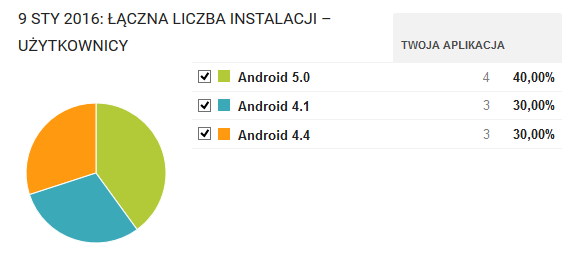
\includegraphics[scale=0.6]{prezentacja_obronaII_zdjecia/wersje_android.png}
			\end{figure}
	\end{frame}
	
		\begin{frame}{Testy beta aplikacji mobilnej - podział instalacji ze względu na wersję aplikacji.}	
			\begin{figure}[H]
				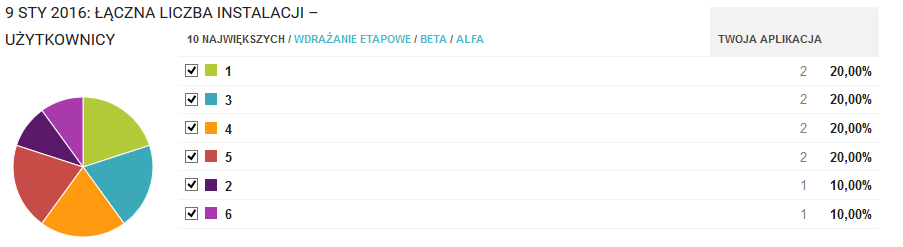
\includegraphics[scale=0.5]{prezentacja_obronaII_zdjecia/wersja_aplikacji.png}
			\end{figure}
		\end{frame}
			\begin{frame}{Wdrożenie aplikacji mobilnej.}	
				\begin{figure}[H]
					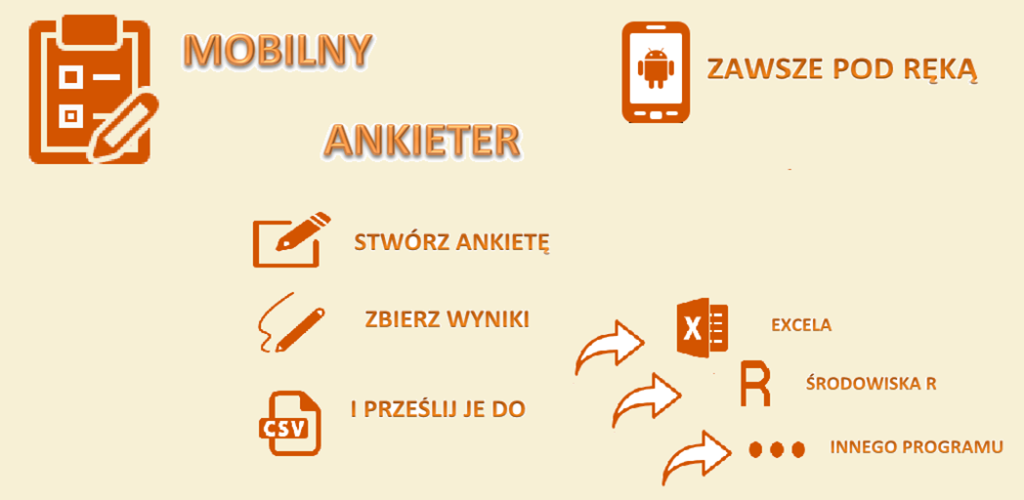
\includegraphics[scale=0.42]{prezentacja_obronaII_zdjecia/baner.png}
				\end{figure}
			\end{frame}
\end{document}